\section{Marco teórico}

En esta sección se desarrollará el funcionamiento teórico de las lanzaderas electromagnéticas, con un enfoque especial en los principios físicos que permiten su operación y la alta eficiencia en el lanzamiento de proyectiles. Comenzaremos con el análisis de los circuitos eléctricos y magnéticos equivalentes del dispositivo, presentando las relaciones principales entre sus componentes. Además, se explicará el circuito de control típico utilizado en estas aplicaciones.

\begin{figure}[h]
    %\centering \raggedleft \raggedright
    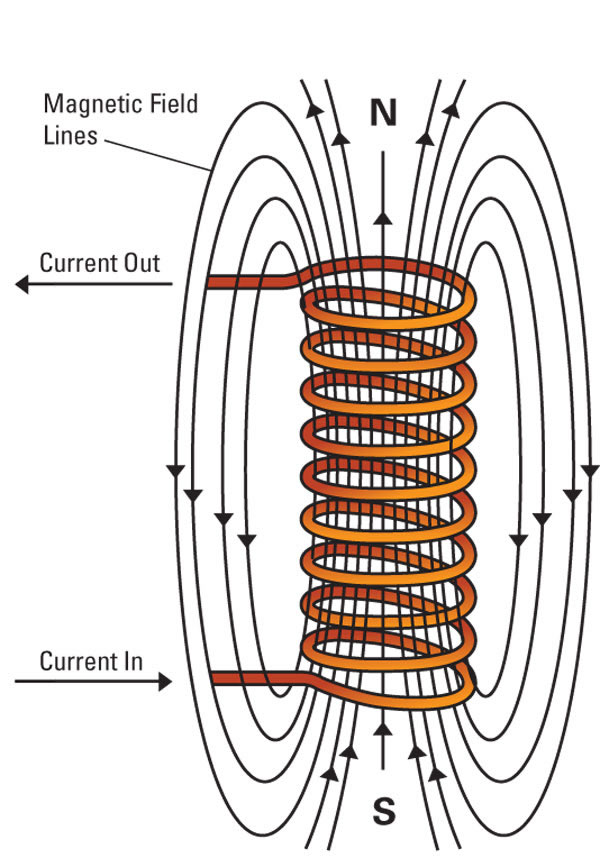
\includegraphics[width=\linewidth]{FigurasMemoria/fig3electromagnet.jpg}
    \caption{Campo magnético en una bobina. www.lanl.gov}
    \label{fig:3} %Para referenciar -> \ref{fig:figNum}
\end{figure}

Como se ha mencionado en la introducción, el funcionamiento de una lanzadera electromagnética se basa en la capacidad de las bobinas de generar un flujo magnético cuando se les aplica una corriente, como se puede ver en la. Esto es debido a la ley de Àmpere, que enuncia lo siguiente:

\begin{quote}
    Según la ley de Ampère, la integral de línea del campo magnético \(\mathbf{B}\) alrededor de un lazo cerrado es igual a \(\mu_0\) multiplicado por la corriente total \(I_{enc}\) que pasa a través de cualquier superficie delimitada por el lazo. Matemáticamente, esto se expresa como:
    \[
    \oint_{\partial S} \mathbf{B} \cdot d\mathbf{l} = \mu_0 I_{enc}
    \]
    donde \(\mu_0\) es la permeabilidad del vacío.
\end{quote}

La manera más básica de representar una lanzadera es un simple circuito con una fuente de alimentación, un interruptor controlado por un circuito electrónico y una bobina, que es la encargada de generar el campo.